\begin{figure}[h!t]
  \begin{center}
    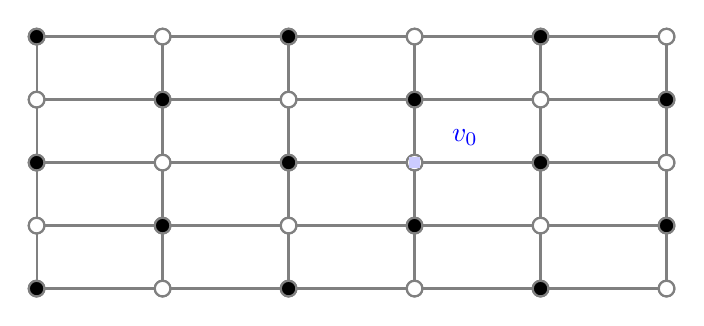
\begin{tikzpicture}[thick, scale=1.6]
      \tikzstyle{every node} = [inner sep = 2pt];
      \foreach \x in {0,...,5}{
        \foreach \y in {0,...,4}{
          \node [draw, circle, black!50] at (\x, \y/2) {};
        }
      }
      \foreach \x in {0,...,4}{
        \foreach \y in {0,...,4}{
          \path[-]
          (\x,\y/2) edge[black!50] (\x+1,\y/2);
        }
      }
      \foreach \x in {0,...,5}{
        \foreach \y in {0,...,3}{
          \path[-]
          (\x,\y/2) edge[black!50] (\x,\y/2 + 1/2);
        }
      }
      \foreach \x in {0,...,5}{
        \foreach \y in {0,...,4}{
          \pgfmathtruncatemacro{\sum}{\x+\y}
          \ifodd\sum
          \node(\x\y) [draw = black!50, circle,fill=white] at (\x, \y/2) {};
          \else
          \node(\x\y) [draw = black!50, circle,fill=black] at (\x, \y/2) {};
          \fi
        }
      }
      \node at (3.4,1.2){\textcolor{blue}{$v_0$}};
      \node[fill=blue!20!white] at (3,1){};
    \end{tikzpicture}
  \end{center}
  
  \caption{Downscaling of the grid graph. Disregarded vertices are filled.}
  \label{fig:downscaling}
\end{figure}